
\thispagestyle{empty} % Die Seite "links" (bei beidseitigem Druck) vom Kapitelbeginn blank machen, wenn sie keinen Inhalt enthält

% % % % % % % % % % % % % % % % % % % % % % % % % % % % % % % % % % % % % % % % % % % % % %
\chapter{Grundlagen}
\thispagestyle{fancy}
\label{kap_grundlagen}

In diesem Kapitel können z.B. die mechanischen Grundlagen der Arbeit genau erläutert werden.

Hier noch ein paar Bsp., wie man zitieren kann:

Wissenschaftliche Artikel in internationalen \textit{journals} oder Fach-Büchern sowie Dissertationen zitiert man so: \cite{Kiefer_Bartel_Menzel_SmartMatStruct_2012,Bartel_Menzel_Svendsen_JMPS_2011,Bartel_Diss}.

Grundlagen der Finite Elemente Methode finden sich in \cite{Bathe}.

Essenzielle Abhandlungen zu Homogenisierungsmethoden werden in \cite{Eshelby01,HashinShtrikman01} beschrieben.

Eines der Grundlagenwerke zur Thermodynamik ist \cite{Truesdell_Noll_01}.

Ein sehr empfehlenswertes Buch zur algorithmischen Behandlung von Nebenbedingungen --- sowohl Gleichungs- als auch Ungleichungsnebenbedingungen --- ist \cite{Bertsekas_01}.

Ebenfalls sehr zu empfehlen ist \cite{Ciarlet_01}, ein Grundlagenwerk zur Kontinuumsmechanik.




Dies ist ein Verweis auf Kapitel~\ref{kap_einfuehrung}.

\newpage

\section{Beispiel für die Einbindung von Bildern}

Text in \texttt{.eps} Bildern kann mittels \verb|\psfrag| in LaTeX übersetzt werden. Dazu werden die Grafiken mit dem \verb|\psfragfig| Befehl eingebunden. Die zu ersetzenden Texte im \texttt{.eps}-Bild können dabei entweder in einer zusätzlichen Datei (hier \texttt{example1-psfrag.tex}) angegeben werden oder direkt hinter dem \verb|\psfragfig| Befehl eingegeben werden. Zu beachten ist dabei, dass Änderungen an den \verb|\psfrag|-Befehlen nur in der extra Datei zu einem automatischen neu kompilieren der Bilder führen. Bei direkter Angabe hinter dem \verb|\psfragfig| Befehl muss im Hauptdokument die Option \verb|pstoolall| an die \verb|iofm_studentthesis| Klasse übergeben werden, oder das entsprechend kompilierte \verb|.pdf| des Bildes (hier \texttt{example2.pdf}) gelöscht werden. Siehe Abbildung~\ref{abb_example}.

\begin{figure}[h]
\centering
    \subfigure[Die Bildunterschrift endet immer mit einem Punkt.]{%
        \psfragfig[width=0.45\textwidth]{Kap02/figures/example1}
    }\hfill
    \subfigure[Die Bildunterschrift endet immer mit einem Punkt.]{%
        \psfragfig[width=0.45\textwidth]{Kap02/figures/example2}{%
            \psfrag{11-cauchy}[l][l]{   ${\scriptstyle \sigma_{11}  }$ }
            \psfrag{11-piolaki}[l][l]{ ${\scriptstyle  S_{11}  }$ }
            \psfrag{Xi-Aust}[l][l]{ ${\scriptstyle \varXi^\A  }$ }
            \psfrag{Xi-Mart}[l][l]{ ${\scriptstyle \varXi^\M  }$ }
            \psfrag{x-kappa}[t][t]{ ${\scriptstyle \text{loading parameter}~\kappa(t)~[-]  }$ }
            \psfrag{y-sig-gpa}[b][t]{ ${\scriptstyle \text{macroscopic stress components}~[\mr{GPa}]  }$ }
            \psfrag{y-xi}[b][t]{ ${\scriptstyle \text{macroscopic volume fraction}~\varXi~[-]  }$ }
            %
            \psr{2}
            \psr{3}
            \psr{4}
            \psr{5}
            \psr{6}
            %
            \pst{1.05}
            \pst{1.1}
            \pst{1.15}
            \pst{1.2}
            \pst{1.25}
            \pst{1.3}
            %
            \psr{0}
            \psr{0.2}
            \psr{0.4}
            \psr{0.6}
            \psr{0.8}
            \psrt{1}
        }%
    }%
    %~ \subfigure[Die Bildunterschrift endet immer mit einem Punkt.]{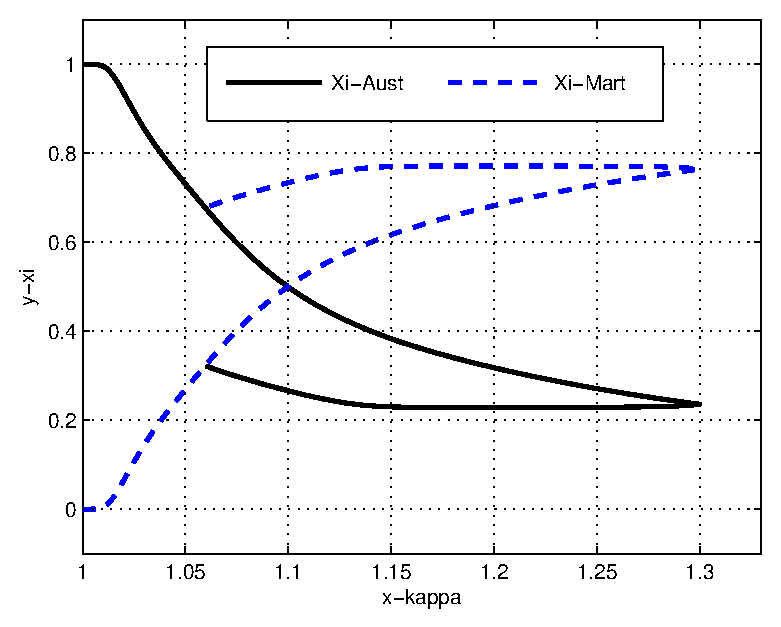
\includegraphics[width=0.45\textwidth]{Kap02/figures/example1.eps}}\hspace{1cm}
    %~ \subfigure[Die Bildunterschrift endet immer mit einem Punkt.]{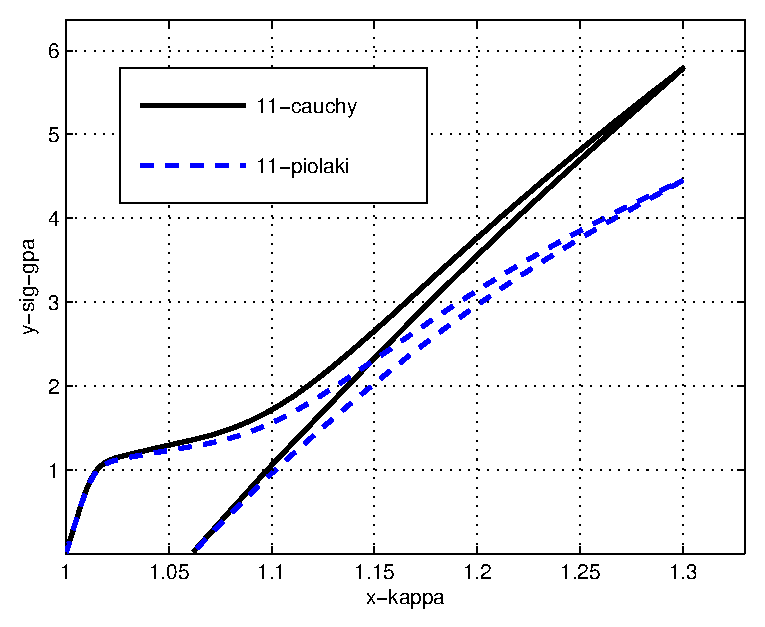
\includegraphics[width=0.45\textwidth]{Kap02/figures/example2.eps}}
    \caption{Mit dem psfrag-Paket lässt sich LaTeX-Schrift direkt in eps-Abbildungen (z.B.~aus Matlab) einbetten. Die Bildunterschrift endet immer mit einem Punkt, siehe auch (a) und (b).}
    \label{abb_example}
\end{figure}



\section{Beispiel für die Einbindung einer Algorithmic Box}

Siehe Algorithmus~\ref{algo_example}.


\begin{algorithm}
    \begin{spacing}{0.7}
        \begin{algorithmic}[1]

            \State given: deformation ${}^{n+1}\B\vareps$ and material state, i.e.~$\left[ {}^{n}\B\xi_i, {}^{n}\B\vareps_{\mr{pl},i}^\mr{1d}, {}^{n}\B\vareps_{\mr{pl,acc},i}^\mr{1d} \right] ~ \forall ~ i \in \{ 1,\dots,n_r \}$
            %           \Comment{  }

            \State set ${}^{n+1}t={}^{n}t+\Delta t \in [\, 0,\, t_\mr{max}\, ]$, initialise ${}^{n+1}\B\sigma = \B 0$ and ${}^{n+1}\BE^\mr{alg} = \B 0$

            \For{ every micro-sphere direction $i = 1 \dots n_r$ }

            \State given: ${}^n\B\xi_i$, ${}^n\B\vareps_{\mr{pl},i}^\mr{1d}$, ${}^{n}\B\vareps_{\mr{pl,acc},i}^\mr{1d}$ at time ${}^{n}t$
            %               \Comment{  }

            \State compute ...
            %               \Comment{  }

            \For{ all combinations $(\alpha,\beta) \in [\mr{A},\Mt,\Mc ], ~\alpha\neq\beta$ }

            \State get energy barriers ${}^{n+1}b_{\alpha\rightarrow\beta,i}$
            %               \Comment{  }

            \State get transformation probabilities ${}^{n+1}P_{\alpha\rightarrow\beta,i}$
            %               \Comment{  }

            \EndFor

            \State assemble ${}^{n+1}\B Q_i$ and obtain ${}^{n+1}\B\xi_i$

            \If{ number of increasing phases $n_\mr{inc}<2$ }

            \State define $\alpha$  as increasing and $\beta$ and $\gamma$ as non-increasing phases

            \State get intermediate plastic strains ${}^n\tilde{\B\vareps}_{\mr{pl},i}^\mr{1d}$

            \Else

            \State define $\alpha$ as decreasing and $\beta$ and $\gamma$ as non-decreasing phases

            \State get intermediate plastic strains ${}^n\tilde{\B\vareps}_{\mr{pl},i}^\mr{1d}$

            \EndIf

            \State get intermediate accumulated plastic strains ${}^n\tilde{\B\vareps}_{\mr{pl,acc},i}^\mr{1d}$

            \State compute intermediate potential $\widetilde{\varPsi}_i = \widehat{\varPsi}_i({}^{n+1}\epsdev_{,i}, {}^{n+1}\epsvol, {}^{n+1}\B\xi, {}^{n}\tilde{\B\vareps}_{\mr{pl},i}^\mr{1d},\theta)$

            \For{ each phase $\alpha$ }

            \State obtain trial plastic driving force ${}^{n+1}q^\alpha_{\mr{pl},\varPsi,\mr{tri}}$

            \If{ for yield function holds $\widehat{\varPhi}^\alpha(q^\alpha_{\mr{pl},\varPsi}, Y^\alpha) > 0$  }

            \State compute Lagrange multiplier ${}^{n+1}\lambda^\alpha$

            \State update ${}^{n+1}\B\vareps_{\mr{pl},i}^\mr{1d}$ and ${}^{n+1}\B\vareps_{\mr{pl,acc},i}^\mr{1d}$

            \EndIf

            \EndFor

            \State add ${}^{n+1}\B\sigma \leftarrow {}^{n+1}\B\sigma + {}^{n+1}\B\sigma_i$ and ${}^{n+1}\BE^\mr{alg} \leftarrow {}^{n+1}\BE^\mr{alg} + {}^{n+1}\BE^\mr{alg}_i$

            \EndFor

            \State return history arrays, i.e.~$\left[ {}^{n+1}\B\xi_i, {}^{n+1}\B\vareps_{\mr{pl},i}^\mr{1d}, {}^{n+1}\B\vareps_{\mr{pl,acc},i}^\mr{1d} \right] ~ \forall ~ i$ as well as ${}^{n+1}\B\sigma$ and ${}^{n+1}\BE^\mr{alg}$

        \end{algorithmic}
    \end{spacing}

    %   } % end of \FontSize
    % ...END FONTSIZE!
    \caption{ Example for an algorithmic box. }
    \label{algo_example}
\end{algorithm}
